\section{Domain Model}

På domain modellen ses det overordnet design af systemet. På figuren tydeliggøres det at al kommunikation mellem server og arduino køre over 3G netværket. Når arduinoen tændes sender den et handshake signal til serveren, signalet fortælle at "den" er online. Efterfølgende pinger arduinoen serveren hvert 30 sekund for at fortælle serveren at den er online. Når serveren modtager handshake fra arduinoen vil dette blive markeret på webapplikationen. Bruger har mulighed for at gemme flyveruter i databasen til senere brug. Billeder taget under flyvning som har fået accept af bruger gemmes i databasen.

\vspace{-5pt}
%kommentar
\begin{figure}[H]
	\centering
	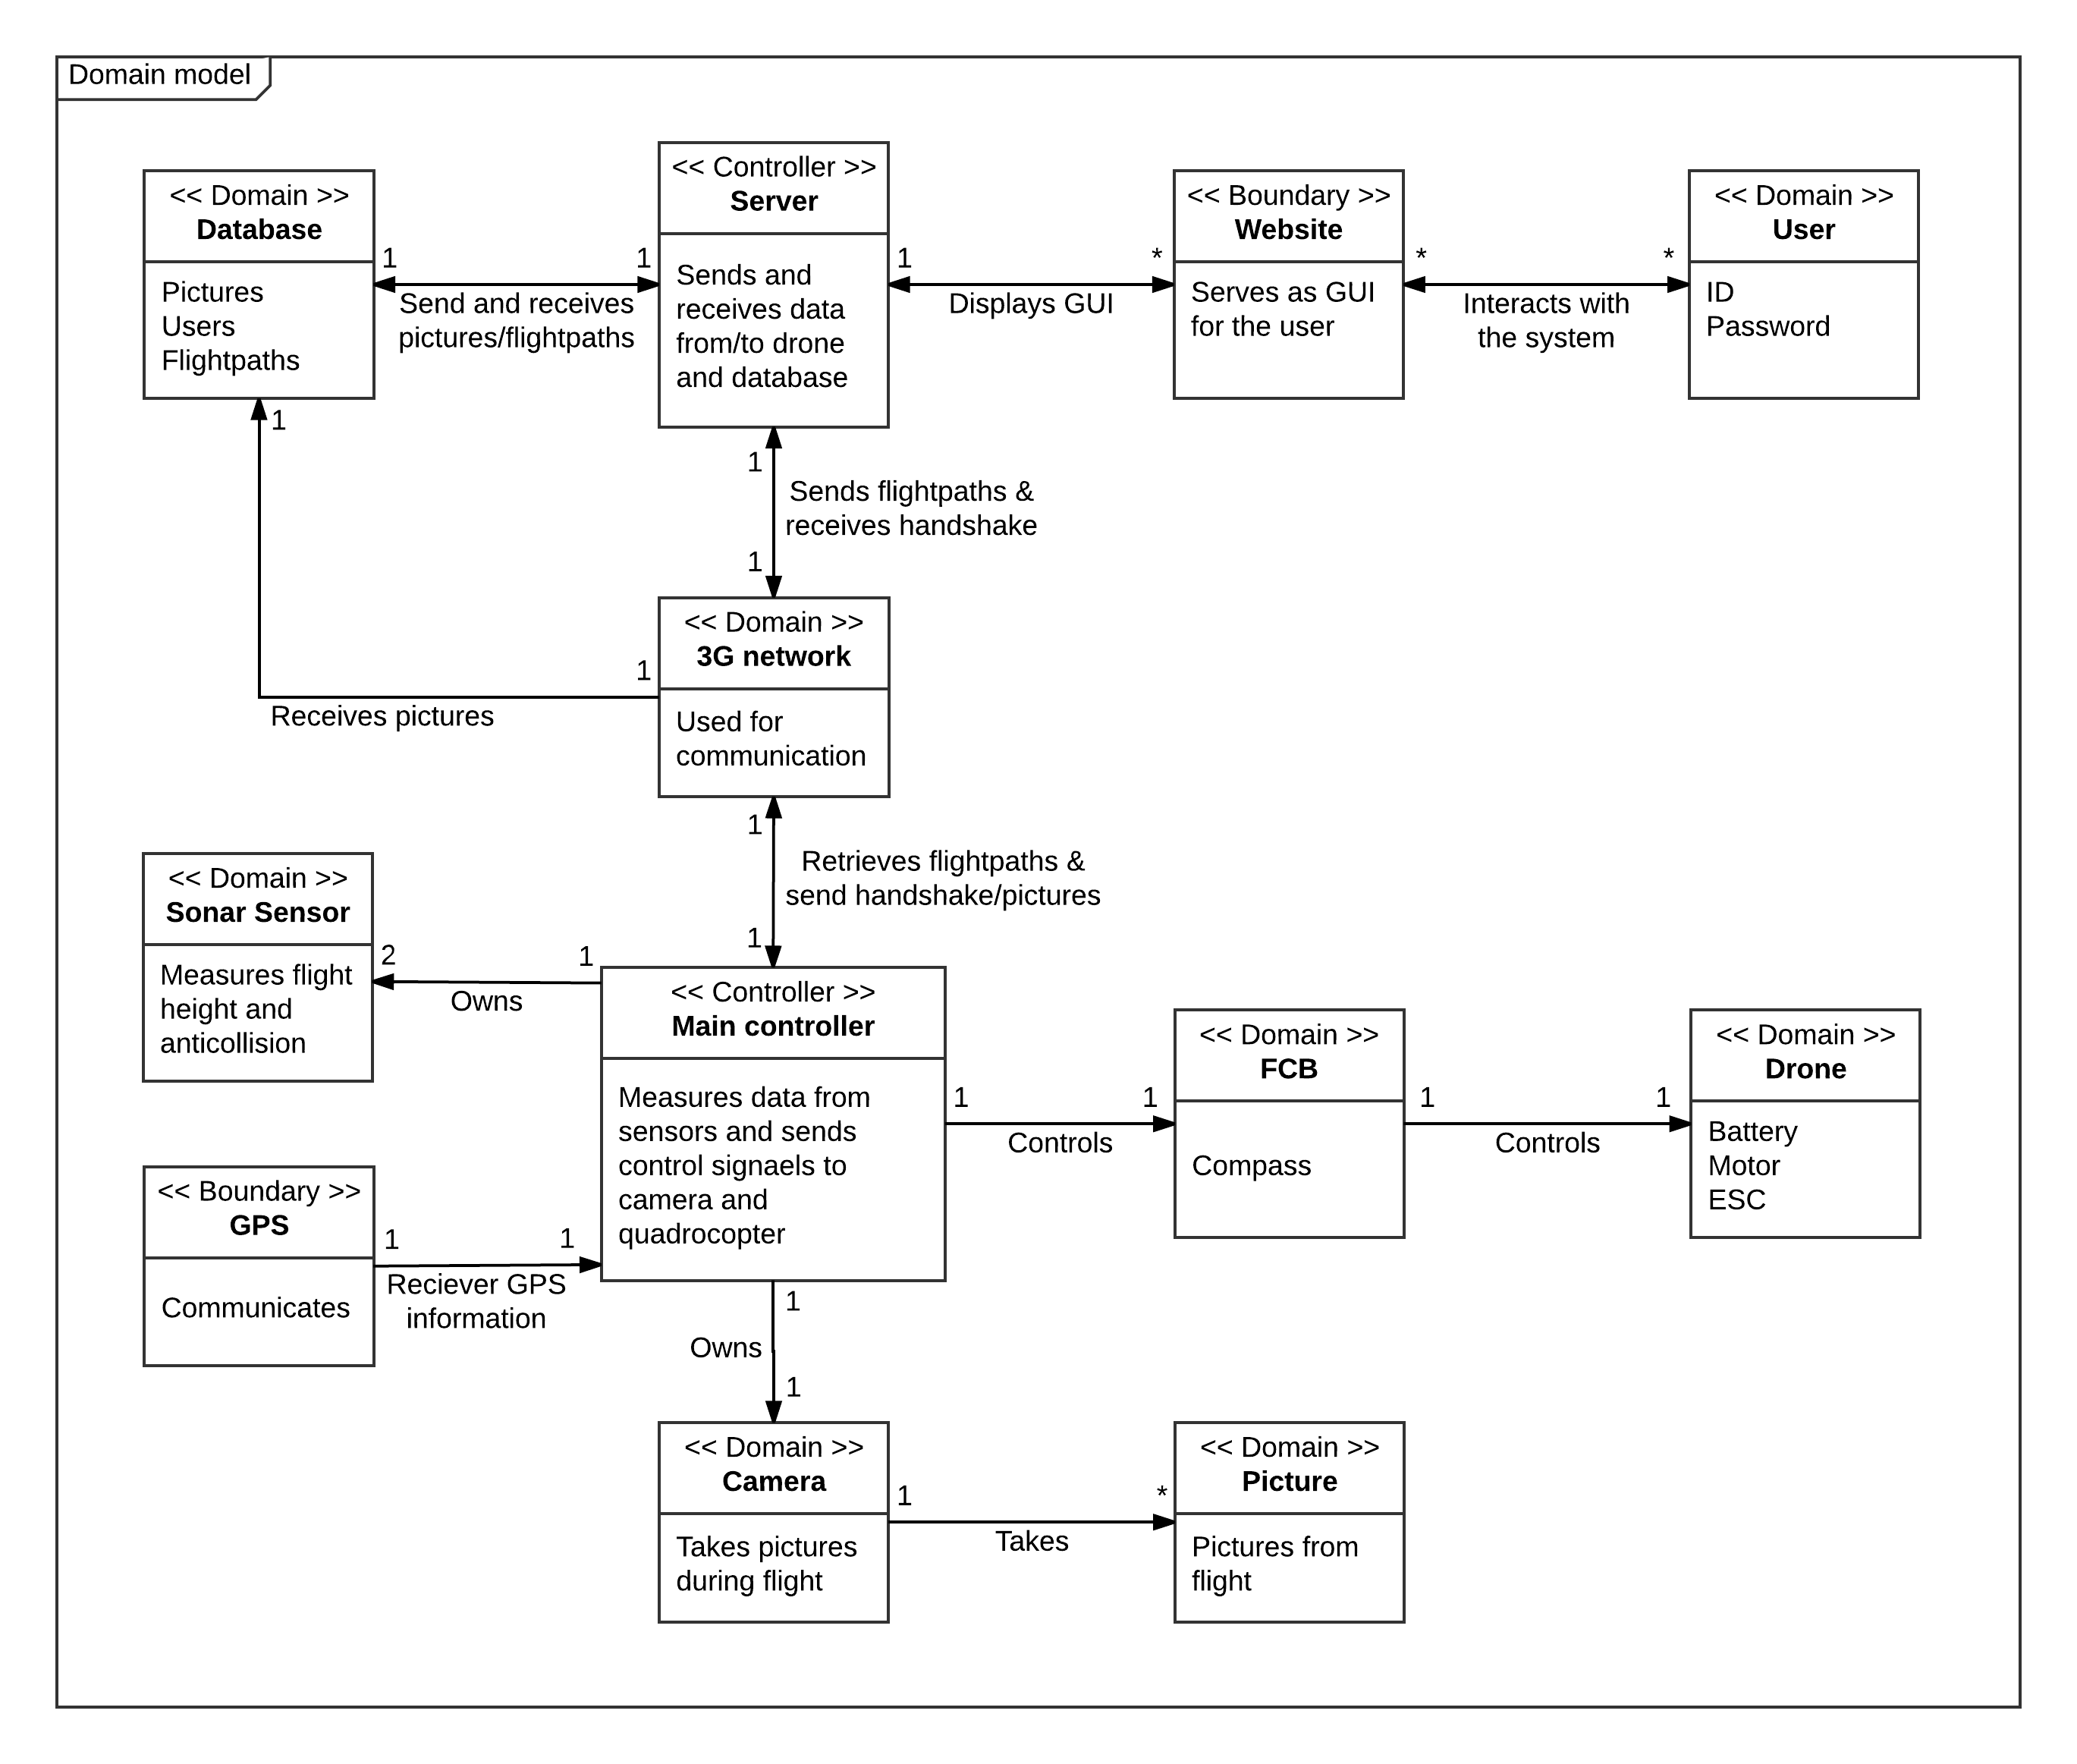
\includegraphics[width=1.\textwidth]{Billeder/domain_model.png}
	\vspace{-5pt}
	\caption{Domain model}
	\label{fig:domain_model}
\end{figure}
